\chapter{Proof of Concept}
\label{ch:poc}

\section{Conway's Game of Life}

Om de compuationele en grafische kant te representeren in een simpele implementatie werd Conway's Game of Life geprogrammeerd met WebGPU. Dit concept werd uitgevoerd op basis van de \textit{codelab} die beschikbaar werd gesteld door google. \autocite{google2023, Qwict2024}

Afbeelding \ref{fig:Conway's Game of Life} geeft de \textit{Conway's Game of Life} implementatie weer hoe deze beschikbaar is op \href{https://gool.qwict.com}{gool.qwict.com}.

\bigbreak{}

\begin{figure}
    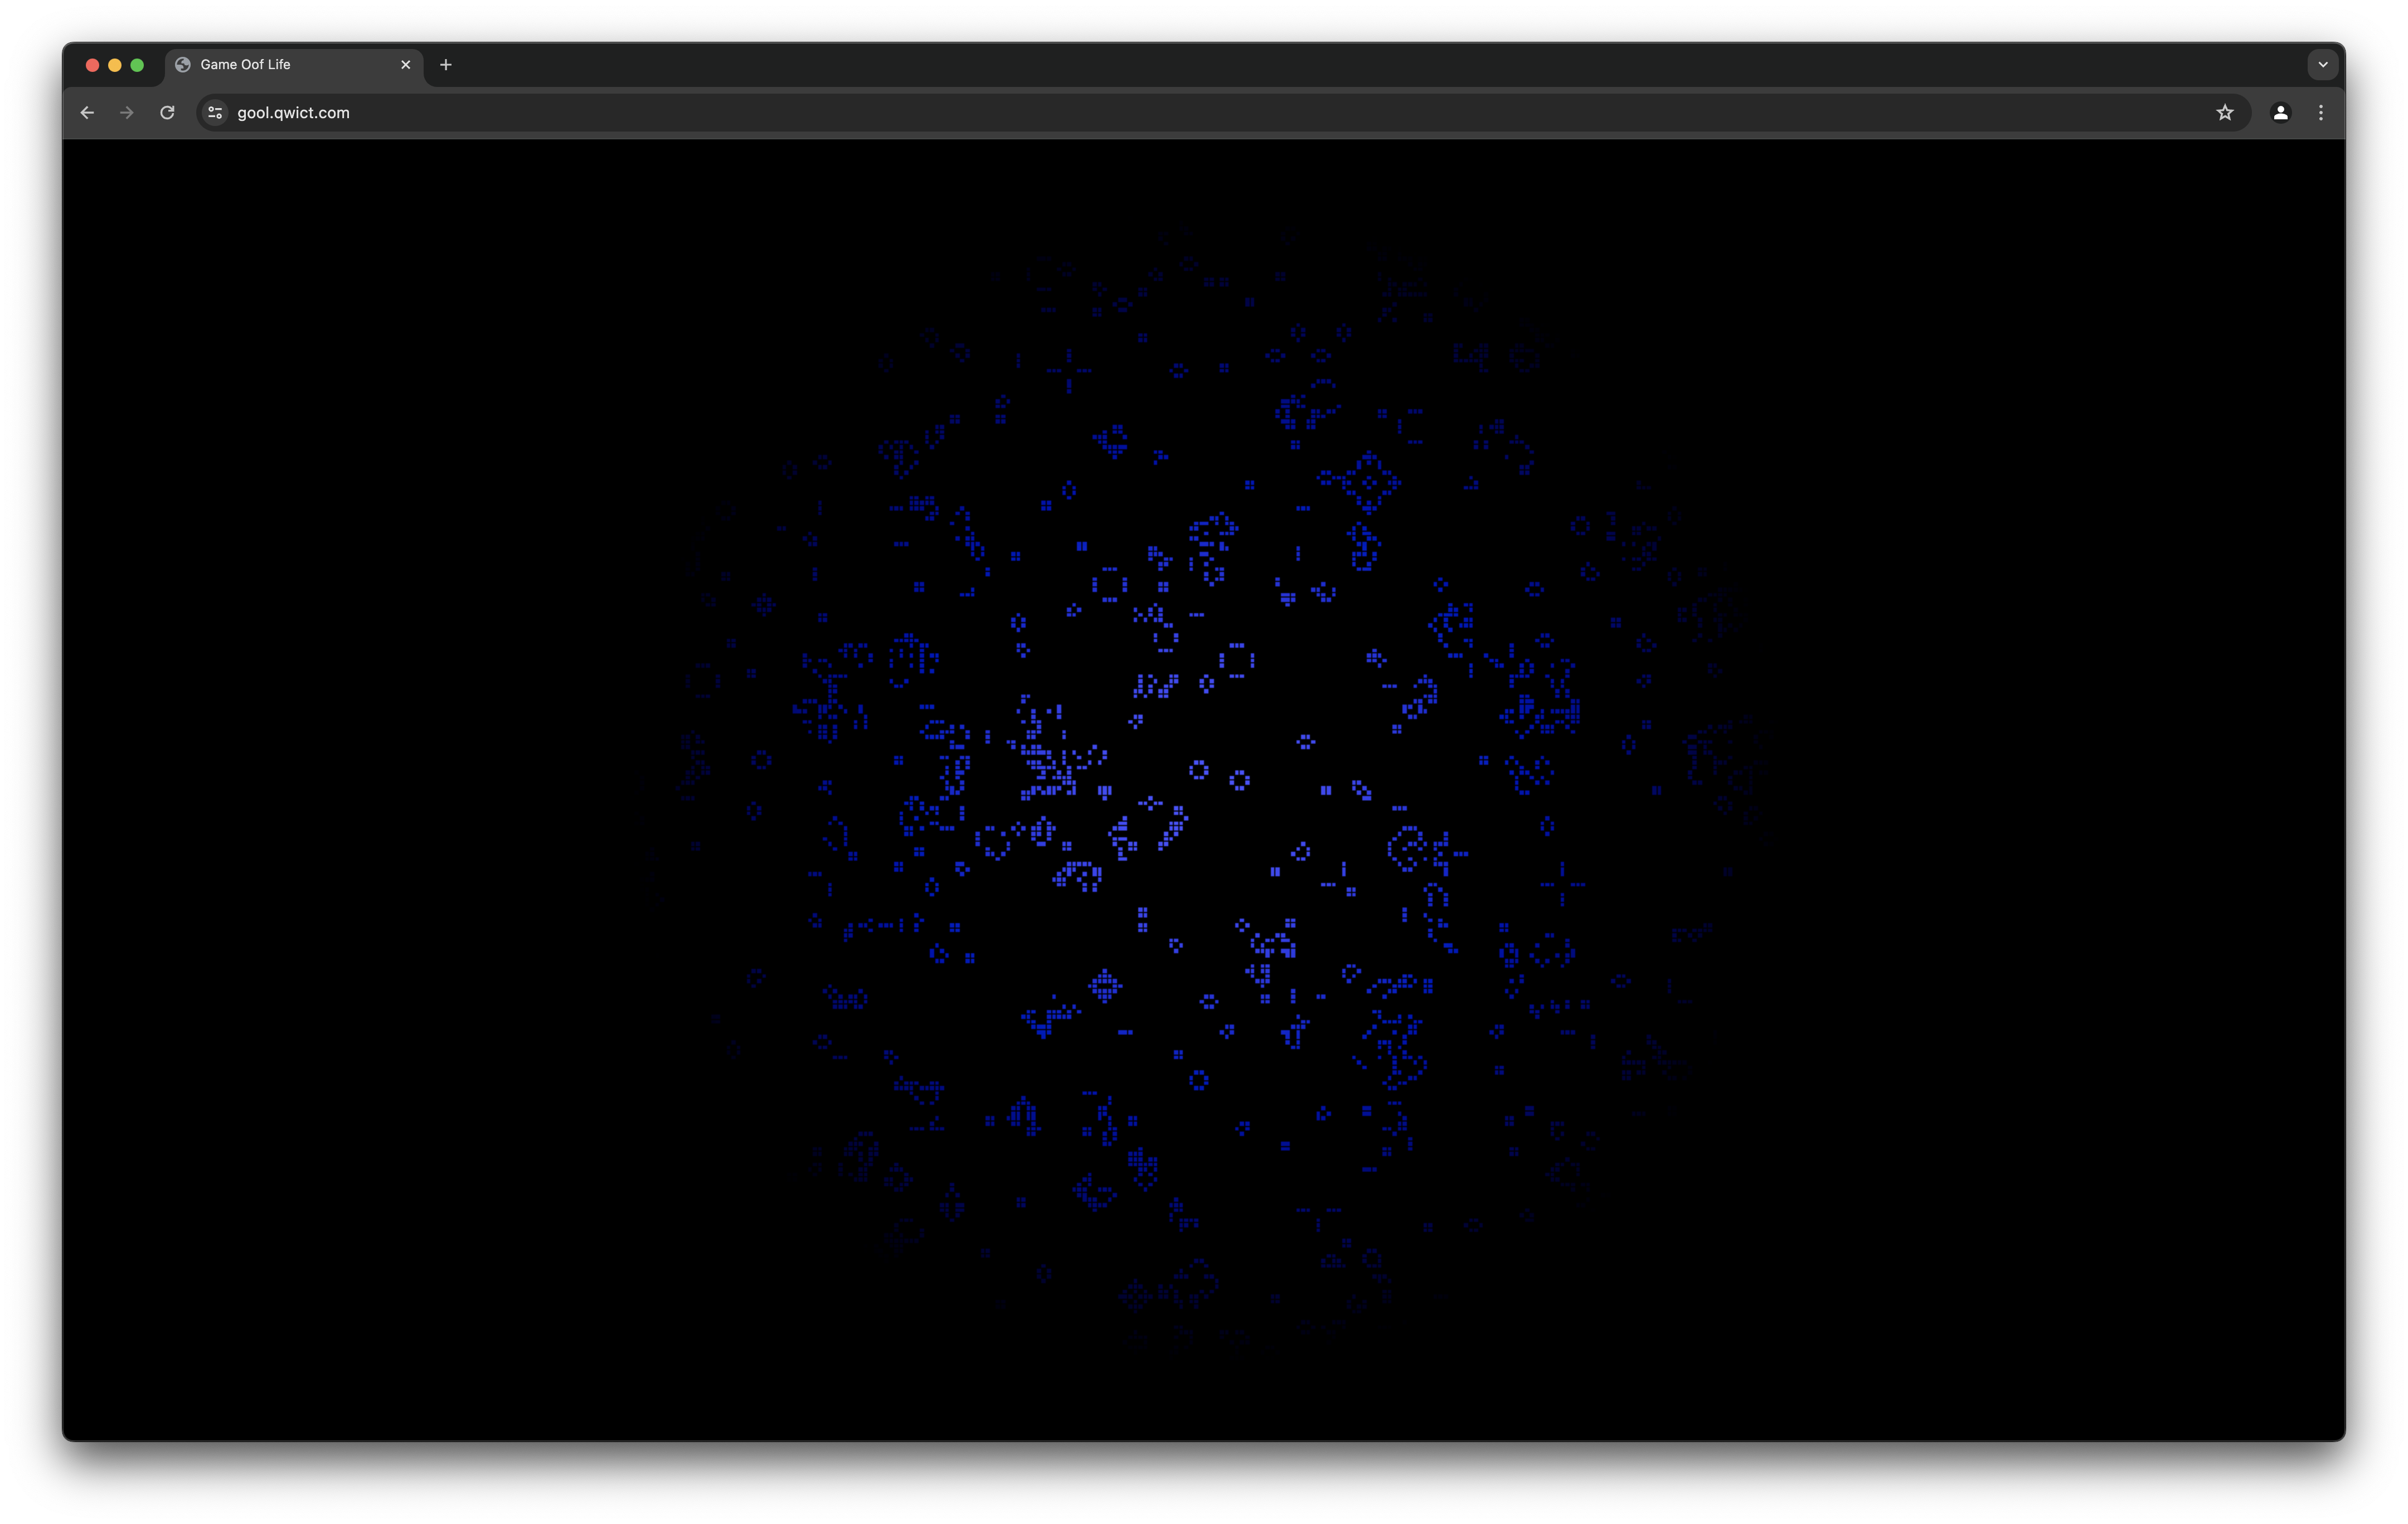
\includegraphics[width=\linewidth]{gool.png}
    \caption[Conway's \textit{Game of Life} implementatie  \autocite{Qwict2024}]{
        Conway's \textit{Game of Life} implementatie beschikbaar op \href{https://gool.qwict.com}{gool.qwict.com}. De broncode is beschikbaar op \href{https://github.com/qwict/GoolWebGPU}{GitHub.com/Qwict/GoolWebGPU}.
    }
    \label{fig:Conway's Game of Life}
\end{figure}

\section{web-llm}

Een implementatie van kunstmatige intelligentie in de browser werd verwezenlijkt door een voorbeeld van \textcite{mlcai2023} aan te passen en hierna te implementeren op eigen server apparatuur. \autocite{Qwict2024a}

\bigbreak{}

Afbeelding \ref{fig:Implementatie web-llm} geeft de \textit{web-llm} implementatie weer hoe deze beschikbaar is op \href{https://chatgpu.qwict.com}{chatgpu.qwict.com}.

\begin{figure}
    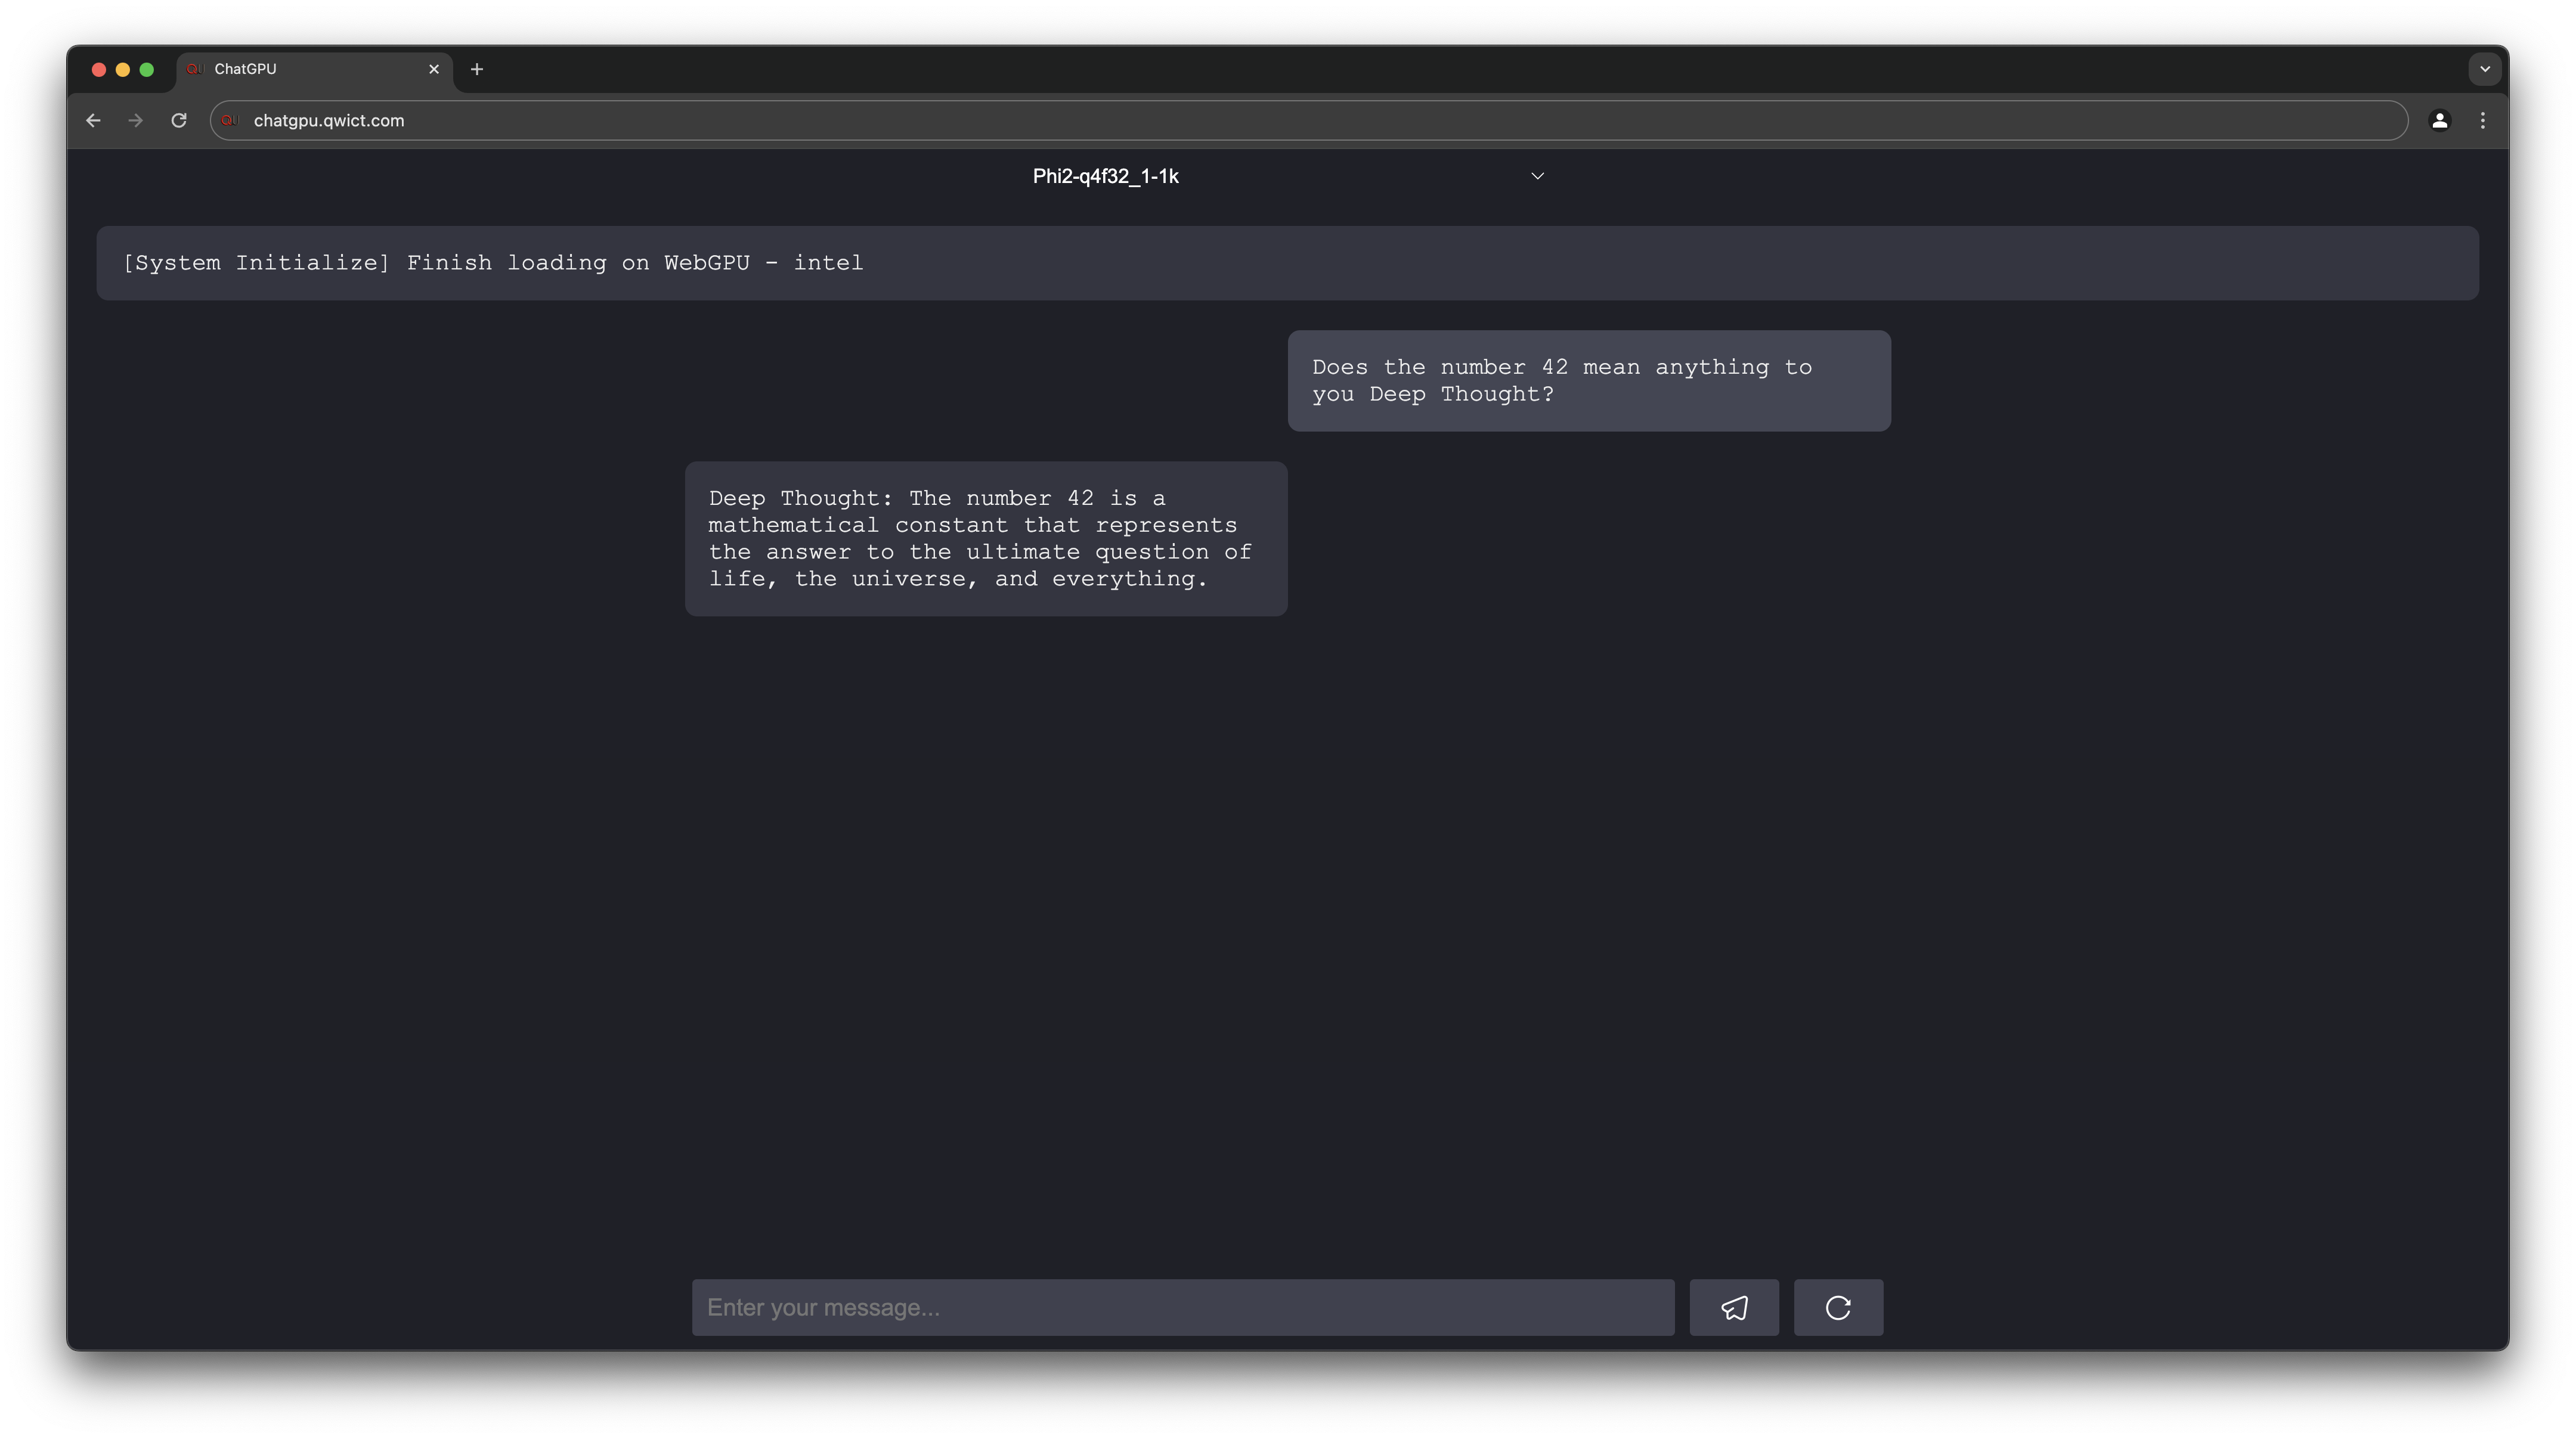
\includegraphics[width=\linewidth]{chatgpu.png}
    \caption[Implementatie web-llm \autocite{Qwict2024a}]{
        Implementatie web-llm beschikbaar op \href{https://chatgpu.qwict.com}{chatgpu.qwict.com}. De broncode is beschikbaar op \href{https://github.com/qwict/chatgpu}{GitHub.com/Qwict/ChatGPU}.
    }
    \label{fig:Implementatie web-llm}
\end{figure}